\documentclass[crop,border={0pt 0 0 0},tikz]{standalone}
\usetikzlibrary{backgrounds,decorations.markings}
\tikzset{>=latex}
\tikzset{->-/.style={decoration={
  markings,
  mark=at position .5 with {\arrow{>}}},postaction={decorate}}}
\begin{document}
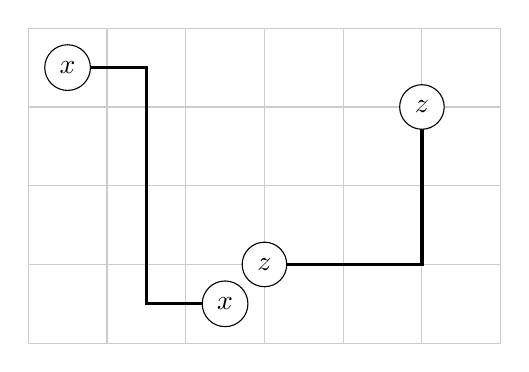
\begin{tikzpicture}
    \draw[step=1, line cap = rect, gray!40] (0,0) grid (6,4);
    
    \draw[black, line cap=rect, very thick] (0.5,3.5) -- +(1,0) -- +(1,-3) -- +(2,-3);

    \draw[black, line cap=rect, very thick] (3,1) -- (5,1) -- (5,3);

    \node[circle, draw ,fill=white] at (0.5,3.5) (x1) {$x$};
    \node[circle, draw ,fill=white] at (2.5,0.5) (x2) {$x$};

    \node[circle, draw ,fill=white] at (3,1) (z1) {$z$};
    \node[circle, draw ,fill=white] at (5,3) (z2) {$z$};


\end{tikzpicture}
\end{document}
